\subsection*{Trunkerings og afrundings problemer}
Mange af de metoder som vi bruger til at udregne, position af det gyldne
snit eller størrelsen af en margin, udregnes med brøker. Hvor i mod et
billedet opbygget af pixels, Dette gør at vi må nød til at tage
approksimationer af udregningerne for at få dem tilbage til et helt tal,
men hvor meget af dataenden er tabt, og hvor maget af resultaterne kan
man stole på.

\subsubsection{Acceptabel afvigelse}
(Nogle referancer)
Som beskravet i kapitel 1, udregnes det gyldne snit med mange decimaler.
En kunstner, selv hvor god han er, har ingen chance for at male så
præcist at man kan sige at strøet ligge nøjagtigt oven på snittet. Vi
starter med at se på alle de ting som kan skabe en usikkerhed fra
mallerns side. Man kan gå ud fra at den procentvise afvigelse ikke er
særlig stor, da de malerier som vi arbejder på kommer fra kunstner som
har være udstillet, dog har vi sat den procentvise afvigelse til 0.5 \%.
Det vil sige at en maller med et lærred på 100 cm, kan male maksimalt
$0.5$ cm forkert.

Nå maleren vælger en ramme og et lærred, har vi igen problemtikken.
Malleren kan være uprecis med sit valg af læret og ramme. Derfor sætter
vi den afvigelse til $1\%$. Da vi igen mener at dette er den maksimalle
afvigelse der kan opstå.

Nå en maller, maller en region i et maleri, forekommerer der normalt en
lille kant rundt og objektet, som et omrids. Dette omrids kan vores
algoritmer ikke tage højte for, og vi må derfor modregne omridset. Nå vi
er sikre at vi ser på ragion og ikke den omrids, Da et omrids ikke er
særligt stor, har vi sat denne procent sats til $0.5\%$. Alt i alt giver
det en afvigelse på vores aktuelde data på $2\%$ det vil sige at nå vi
finder en region i billedet som ligger på pixel 200, og et billedet som
er $500$ bredt, befinder den sig faktisk i intervallet [190,210]. Måden
vi tager højte for den forskel, er ved hjælp af marginer, som er afsnit
$2.2$.

Vi regner med procenter, som godt kan være lidt misvisende, da det
afhænger af billedets størelse, et billedet som er meget stort, kan
malleret male meget ved siden af, i forhold til en lille billedet. Men
da vi gerne vil have at løsningen er dynamis, er procenter den beste
variabel.

\subsection{Hvordan deles billedet efter snittet}
I billedet bliver højde og breaden betegnet som $H$ og $B$, se figur
\ref{cut}. Der er 4 snit i billederne 2 vertikale og 2 horisontale, i
figur \ref{lenasnit2} er de 4 gyldne snit tegnet ind. For at finde ud af hvor
de 4 snit skal ligge i billedet multipliseres B og H med $\varPhi$ som
giver to tal som betegner, hvor mange pixels fra begge kanter, det
gyldne snit befinder sig f.eks ved et billedet, som har $B = 4000$ pixel,
vil snittet ligge ved, $4000 \cdot \varPhi \approx 2472$.

\begin{figure}[h]
	\begin{center}
		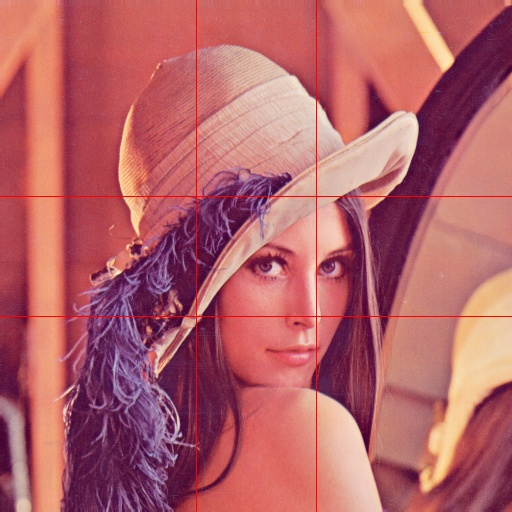
\includegraphics[scale=0.42,angle=0]{afsnit/vores_implementation/billeder/naiv_algoritme/Lenagolden}
	\end{center}
	\caption[]{Billedet som har indtegnet de fire gyldne snit}
	\label{lenasnit2}
\end{figure}

\begin{figure}[h]
	\begin{center}
		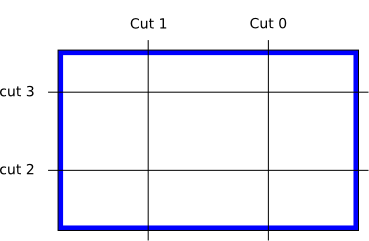
\includegraphics[scale=0.42,angle=0]{afsnit/vores_implementation/billeder/naiv_algoritme/Cut}
	\end{center}
	\caption[]{Billedet hvor de 4 snit er navngivet og højden og breaden}
	\label{cut}
\end{figure}

De 4 snit blivre tildelt vært deres id, snit 0,3 som de vil bliver
refereret til i reste af raporten. hvis vi i steden for de gyldne snit
vil finde et snittet 0.5 bliver der kun skabe 2 cut i steden for firere.
id for disse 2 snit er snit 0 og snit 1. ilustret i figur \ref{2Cut}.

\begin{figure}[h]
	\begin{center}
		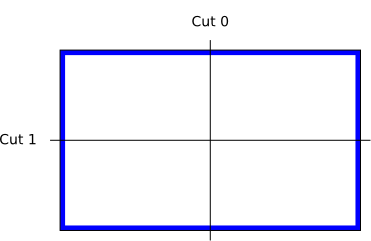
\includegraphics[scale=0.42,angle=0]{afsnit/vores_implementation/billeder/naiv_algoritme/2Cut}
	\end{center}
	\caption[]{billedet bliver kun skøret af 2 snit}
	\label{2Cut}
\end{figure}

\subsubsection*{Heltal i det gyldne snit}

Eksemplet med 4000 pixels ovenfor, approksimerer vi antal pixels ved at
afrunde resultatet, se udregning \ref{afrundning}. Det gør at vi mister
0.13595 nøjagtighed, hvilket svare til en misvisning af punktet på
0.00339875 $\%$ i forholdt til bredden på billedet. se udregnig
\ref{afrundning2}. 

\begin{equation}
	4000 \cdot \varPhi = 4000(\sqrt{5}-1)/2 = 2472.13595 \approx 2472 \label{afrundning}
\end{equation}

\begin{equation}
	0.13595/4000 \cdot 100 = 0.00339875 \label{afrundning2}
\end{equation}

Det er en maget lille del af selve billedet og skulle ikke give nogle
misvisninger i forhold til udregningen. For at gøre det lidt mere
generadt, sætter vi trunkeringsfejlen til $0.5$, da det er den maximale
afrundings factor som kan forekommer. Hvis billedet har en størrelse på
500 pixels, som er det miste billedet vi har, dette giver en fejl margen
på $0.1\%$, Dette tal bliver adderet til fejl satsen ovenfor, og giver
en samlet afvigelse på $2.1\%$

\subsubsection{Heltal ved udregning af Margin}
Når vi har 2 snit, F.eks. ved $\varPhi$ og $\frac{2}{3}$ som skal sammenligne og
som ligger meget tæt på hinanden, er det vigtigt at margin for vært
snittet ikke krydser hinanden. Hvis margin krysser vil det indebære at de samme region
vil blive fundet af begge snit, og vil give et skævt billedet af
forskellen på de to snit. Derfor må vi sørge for at de margin ikke
krydser. hvis $x$ betegner antal pixels i $B$ eller $H$, og vi vil se
forskellen mellem $\frac{2}{3}$ og $\varPhi$, multiplicere vi $x$ med snittet for at
finde dens placering og subtrahere dem fra hinanden.

\begin*{eqnarray}
	\frac{x2}{3}-\frac{x2}{\sqrt{5}+1} &=& x(\frac{2}{3}-\frac{2}{\sqrt{5}+1}) \\ \nonumber
	&=& x(0.666667-0.618034) \\ \nonumber
	&=& x(0.048633) \\ \nonumber
\end*{eqnarray}

Vi har nu fundet antal pixels mellem de to snit. Vi vil gerne undgå at
de to marginens ikke krydser hinanden, så der dividere vi med 2 og
afrunder verdien.

\begin{equation}
	\lfloor \frac{0.048633x}{2}\rfloor = \lfloor0.024316x \rfloor
\end{equation}

Tallet $2.4316$ er altså den minimale procentvise størelse som vores
margin må have, nå vi sammen liner det gyldne snit og $\frac{2}{3}$.
Det betyder også at vi ikke må sammen line snit som ligger særlig
meget tætter på hinanden, da 0.021 er den minimale procent margin som vi må have.
$\lfloor 0.024316x \rfloor$ giver os et antal pixels som skildre de to snit. For at vise
hvor stort marginen egentlige kan være, bruger jeg denne formel på to
billeder, et som svare til vores mindste billedet, 500 pixels, og et
som svare til vores største billedet, 4000 pixels. Ved 500 pixels
bliver resultatet

\begin{equation}
	 \lfloor 500(0.024316)\rfloor = 12
\end{equation}

Det er en fint margin, da vores fejl på udregningerne ligger på 2.1 \%,
som svare til $\lseil 500*0.021 \rseil = 11$ pixels, som er 1 pixels fra vores
margin

Ved 4000 pixels giver det.

\begin{equation}
	 \lfloor 4000(0.024316)\rfloor = 97
\end{equation}

Som også er god nok da $4000*0.021 = 84$ pixels. Vi har valt at bruge
$2.4\%$ som vores minimum margin procentiv og ikke 2.1 da vi gerne
vil have en margin som er lidt støre en den teoratiske fejl margin.
\label{margin}
% vim: set tw=72 spell spelllang=da:
